\documentclass[12pt,a4paper]{article}
\usepackage[french]{babel}
\usepackage[T1]{fontenc}
\usepackage[utf8]{inputenc}
\usepackage{tabto}
\usepackage {graphicx}
\usepackage{color}
\usepackage{hyperref}

\begin{document}

    \begin{figure}
 
        
\includegraphics[width=4cm]{images/logolemansU.png}
        \hspace{150pt}
        
\includegraphics[width=4cm]{images/logo_IC2.png}
        
    \end{figure}
    
    \title{
        \color{blue}\textbf{Le Mans Université}\\
        \color{black}Licence Informatique \textit{2ème} année\\
        Module 174UP02 Rapport de Projet\\
        \textbf{MétaTravers}
    }
    
    \author{Bossard Guilian\\Mezrhab Bilal\\Perron Nathan}
    \date{\today}
    \maketitle
    \begin{center}
        \href{https://github.com/Slyolas/projetL2.git}{Lien vers notre GitHub}
    \end{center}
    \newpage

    \tableofcontents

    \newpage

    \section{Introduction}
        \tabto{1cm} Ce rapport présente le travail accompli dans le cadre de notre projet de fin d'année en deuxième année d'informatique. Notre objectif principal était de concevoir et de développer un jeu, exploitant les compétences acquises au cours de notre formation. \\
        
            \tabto{1cm} Notre jeu est inspiré de l'univers de «~Mario Bros~», où chaque niveau offre un mini-jeu unique et palpitant. Vous incarnez un personnage intrépide qui traverse ces niveaux, affrontant des pannes système, des virus informatiques et d'autres obstacles numériques. L'objectif est de résoudre les problèmes et de restaurer l'intégrité des systèmes informatiques, tout en explorant des paysages virtuels colorés et imaginatifs. Avec des mécaniques de jeu simples et intuitives, cette aventure promet une expérience accessible et amusante pour les joueurs de tous âges et de tous niveaux.\\\\
             
            \tabto{1cm} Chaque défi offre une expérience unique et mémorable, des environnements de bureau traditionnels aux mondes numériques fantaisistes, en passant par des défis de réflexion, d'adresse et de vitesse. Avec une grande diversité de niveaux et de mini-jeux, cette aventure propose une expérience sans cesse renouvelée, où chaque étape apporte son lot de surprises et de découvertes. Mêlant action et résolution de problèmes, notre projet offre une expérience de jeu riche et engageante qui saura captiver les joueurs du début à la fin.
            
        \subsection{Description des mini-jeux}
        
            \begin{itemize}
            
                \item \tabto{1cm} \underline{Niveau 1 - Découverte du jeu :} \\\\
                \tabto{1cm} Ce premier niveau offre une introduction simple des mécaniques de déplacements de «~MétaTravers~». Les joueurs seront plongés dans un environnement virtuel sobre mais engageant, où ils auront l'occasion de se familiariser avec les commandes de base du jeu. Des obstacles simples mais significatifs seront présents pour guider les joueurs à travers cette première étape de leur aventure.\\
                
                \item \tabto{1cm} \underline{Niveau 2 - Problème de refroidissement :}\\\\
                \tabto{1cm} Dans ce niveau, les utilisateurs seront confrontés à un défi technique crucial~: un problème de refroidissement menace la stabilité de la machine principale. Inspiré du concept du jeu «~Pipe~», ce niveau mettra à l'épreuve les compétences des joueurs pour reconfigurer efficacement le réseau de conduits de refroidissement. Des obstacles supplémentaires et des contraintes de temps seront ajoutés pour augmenter la tension et l'urgence de la situation.\\

                \item \tabto{1cm} \underline{Niveau 3 - Invasion de virus :}\\\\
                \tabto{1cm} Le système est submergé par une vague de virus informatiques. Les utilisateurs devront faire preuve de rapidité et de précision pour éliminer les virus tout en protégeant les données vitales du système. Des mécaniques de combat simples vues au premier niveau seront de retour pour permettre aux joueurs de repousser cette menace numérique.\\
                
                \item \tabto{1cm} \underline{Niveau 4 - Reconstruction critique :}\\\\
                \tabto{1cm} Ce niveau mettra à l'épreuve la capacité des utilisateurs à résoudre des puzzles et à utiliser leur créativité pour reconstruire une pièce essentielle du système. Les joueurs devront collecter et assembler des composants dispersés dans l'environnement pour restaurer la fonctionnalité du système. Un défi unique pour ajouter de la profondeur et de l'intérêt à cette tâche.\\

                \item \tabto{1cm} \underline{Niveau 5 - Déplacement de données :}\\\\
                \tabto{1cm} Bienvenue dans un labyrinthe numérique complexe où les utilisateurs doivent naviguer à travers une multitude de passages étroits et de chambres pour déplacer des données cruciales d'un point à un autre. Des énigmes de logique et des obstacles variés seront présents pour défier les joueurs tout au long de leur mission. La planification stratégique sera essentielle pour atteindre la destination finale.\\


                \item \tabto{1cm} \underline{Niveau 6 - Évasion du monde virtuel :}\\\\
                \tabto{1cm} Vous avez atteint le dernier niveau de «~MétaTravers~» ! Dans ce défi final, les utilisateurs devront utiliser toutes les compétences et les connaissances acquises au cours de leur aventure pour trouver un moyen de sortir de ce monde virtuel et de revenir à la réalité. Les obstacles seront plus complexes et les enjeux plus élevés que jamais. Seuls les joueurs les plus déterminés et les plus habiles réussiront à surmonter ce dernier défi et à échapper à ce monde numérique.
                
            \end{itemize}

    \section{Organisation du travail de chacun}
        \tabto{1cm} La création du groupe s'est déroulée de manière naturelle, basée sur les affinités de chacun et sur la motivation commune envers le projet. Chaque membre était conjointement motivé et prêt à s'investir dans le travail nécessaire à fournir.

        \subsection{Émergence du projet}
            \tabto{1cm} Le processus d'émergence du projet a été marqué par des discussions approfondies concernant le type de jeu à développer ainsi que son déroulement. Initialement, l'idée de concevoir un jeu dans le style de «~Mario Bros~», avec des plateformes et des ennemis, était prédominante. Cependant cette approche a rapidement été remise en question, car elle ne permettait pas d'incorporer suffisamment d'éléments personnalisés. C'est ainsi qu'est née l'idée novatrice de créer une série de mini-jeux tout en préservant l'essence du concept initial, offrant ainsi une expérience plus riche et variée aux joueurs.\\

            Dans notre quête d'insérer une touche personnelle distinctive dans le jeu, nous avons entrepris une reflexion approfondie sur la trame scénaristique et les personnages. Diverses idées ont été explorées, telles que la réinvention de l'histoire de «~Mario Bros~» ou la création d'un univers fantaisiste. Cependant, nous avons opté pour une approche innovante en choisissant un concept lié à l'informatique, où le personnage principal voyagerait à travers les systèmes pour les réparer. L'idée d'un agent spécial revêtant un costume et des lunettes de soleil est apparue comme une évidence, symbolisant son engagement dans des missions complexes et risquées, à l'instar de «~Neo~» et de «~Trinity~» dans «~Matrix~».\\

            La phase de conception du jeu a également nécessité la recherche d'un nom évocateur. Après un début animé et la proposition de nombreuses idées, le nom «~MétaTravers~» a été retenu. Cette appelation incarne parfaitement notre concept, symbolisant le voyage à travers les différentes dimensions numériques pour atteindre nos objectifs.\\
            
        \subsection{Répartition des tâches}
            \tabto{1cm} Concernant la répartition des tâches, nous avons opté pour une approche méthodique et équilibrée. À cette fin, nous avons utilisé un diagramme de Gantt pour planifier et attribuer les différentes responsabilités en fonction des compétences et des disponibilités de chaque membre de l'équipe.\\Parrallèlement, l'utilisation de GitHub comme plateforme de collaboration a grandement facilité l'échange des données et la gestion du travail en permettant à chacun de contribuer de manière transparente et organisée.\\Malgré quelques écarts par rapport au planning initial, notre approche flexible, basée sur des réunions régulières et une communication ouverte, nous a permis de maintenir un niveau élevé d'efficacité et de cohésion au sein de l'équipe.\\

            Dans un souci d'équité et d'efficacité, chaque membre s'est vu attribuer des tâches en fonction de ses compétences, de ses envies, et de la dureté des tâches. Cette approche a permis de garantir que chacun puisse contribuer de manière significative au projet, tout en assurant une répartition équilibrée de la charge de travail. De plus, la mise en place d'un système de suivi des tâches et de leur avancement a permis à chacun de rester informé et engagé dans le processus, renforçant ainsi notre collaboration et notre cohésion en tant qu'équipe.\\

            \begin{figure}[h]
                \centering
                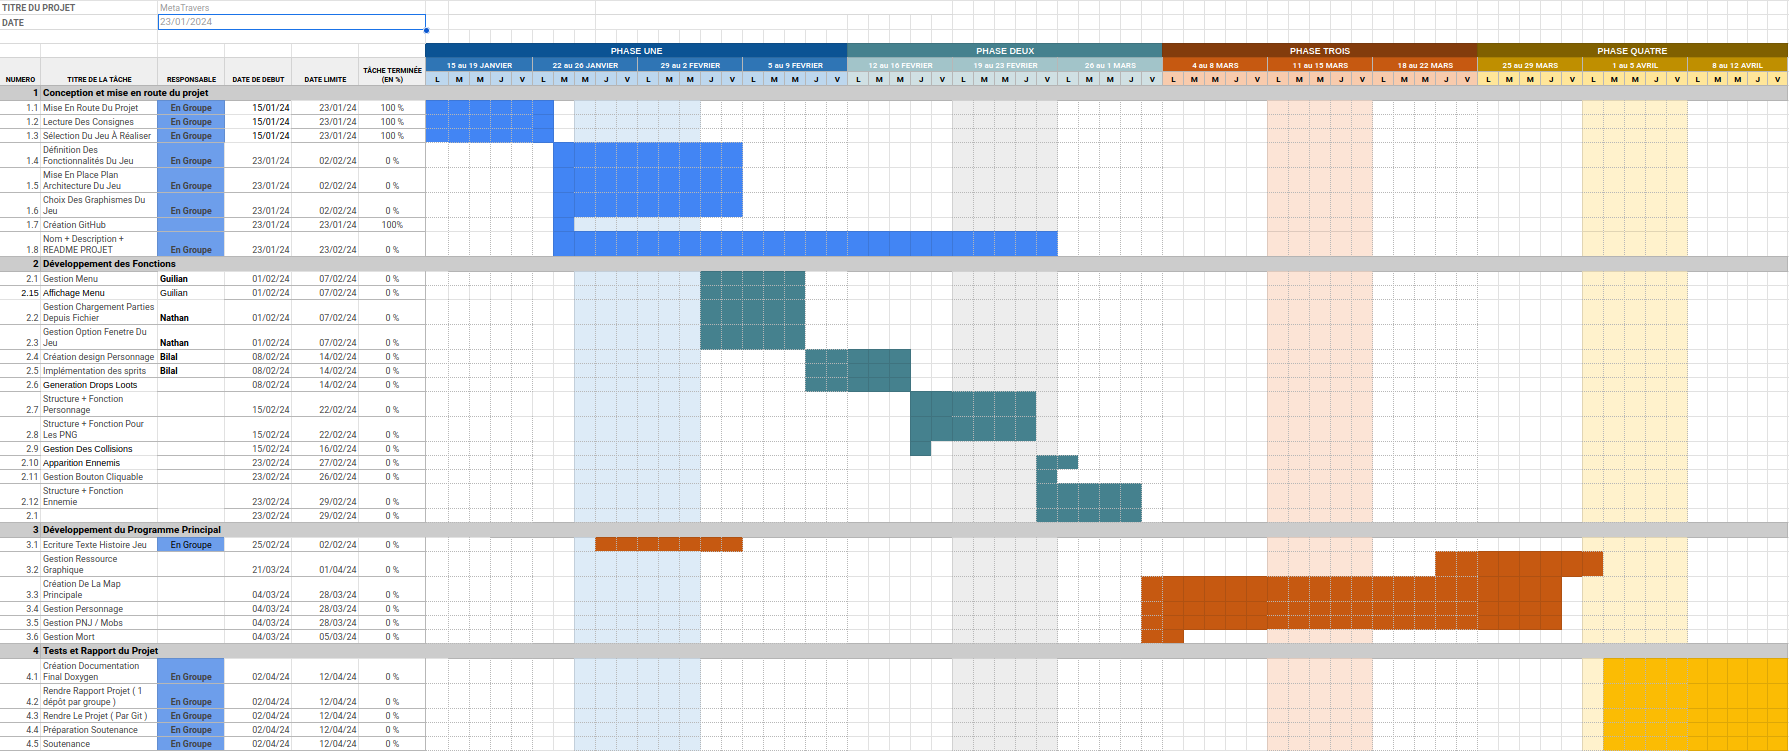
\includegraphics[width=13cm]{images/diagramme_GANTT.png}\\
            \end{figure}

    \newpage
    
    \section{Analyse et conception du projet}
        \tabto{1cm} Dans cette seconde partie, nous allons présenter ce que nous avons fait au début du projet juste après avoir décidé du style de jeu que nous allions faire. Nous avons analysé le problème que l'on devait traiter, c'est à dire réfléchir aux différentes règles du jeu et aux fonctionnalités disponibles pour le joueur. Par la suite, nous avons réfléchi à la conception des différents onglets présents dans le jeu. On peut notamment y retrouver le menu principal, les options, etc.

        \subsection{Analyse du projet}
            \tabto{1cm} Nous avons donc décidé de créer un projet dans le même style que les jeux «~Mario Bros~» qui possèdent des règles de jeu relativement simples. Le but de notre jeu est d’arriver à la fin des quatre niveaux différents en essayant de récupérer un maximum d’objets et de mourir le moins de fois possibles. Chaque niveau possède trois objets différents, parfois très bien cachés ou très difficiles à récupérer ce qui pousse le joueur à bien explorer tous les recoins du jeu et à prendre des risques.\\

            \tabto{1cm} De plus, notre jeu possède différentes fonctionnalités pour que tous les joueurs puissent jouer dans les meilleures conditions possibles et avoir un confort de jeu optimal. Notre projet possède une navigation simple qui permet aux utilisateurs même débutants de ne pas se perdre dans les menus ou dans le jeu. Notre jeu est composé de différentes pages qui représentent des onglets différents. On peut y retrouver les onglets du menu principal, de la création d’une nouvelle partie, des options, de la carte où l'utilisateur va pouvoir jouer au niveau qu'il souhaite et bien sûr les onglets des quatre niveaux, sans compter l’introduction lorsque l'on commence une nouvelle partie.

        \subsection{Conception du projet}
            \tabto{1cm} Nous avons donc divisé notre jeu en plusieurs onglets qui possèdent tous différentes fonctionnalités pour que les joueurs puissent y naviguer facilement.\\

            \begin{itemize}
            
                \item \tabto{1cm} \underline{Le menu principal~:} \\\\
                \tabto{1cm} Cet onglet est le tout premier qui s’affiche quand l’utilisateur lance le jeu, il est composé d’un fond d’écran qui représente le thème de notre projet, son titre et de plusieurs boutons cliquables. Ces derniers permettent de continuer la partie s’il en existe déjà une, de créer une nouvelle partie si le joueur veut recommencer le jeu ou bien d’accéder aux différentes options mises à disposition.\\

                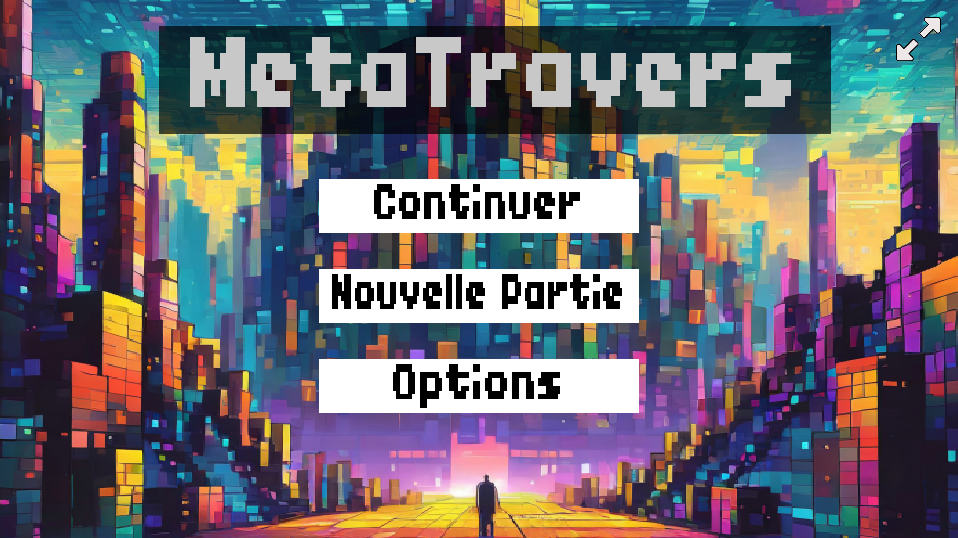
\includegraphics[width=10cm]{images/menu_principal.png}\\
                
                \item \tabto{1cm} \underline{La nouvelle partie~:}\\\\
                \tabto{1cm} En cliquant sur le bouton « Nouvelle partie », le joueur accède à une
                nouvelle page où il pourra recommencer le jeu du début. Il aura la possibilité de choisir différents paramètres comme son pseudonyme, son personnage entre un homme et une femme et le mode de jeu. Il existe le mode normal qui est accessible par tous les joueurs quel que soit leur niveau et un mode difficile qui est réservé aux personnes qui connaissent bien le jeu et qui cherchent un défi supplémentaire.\\

                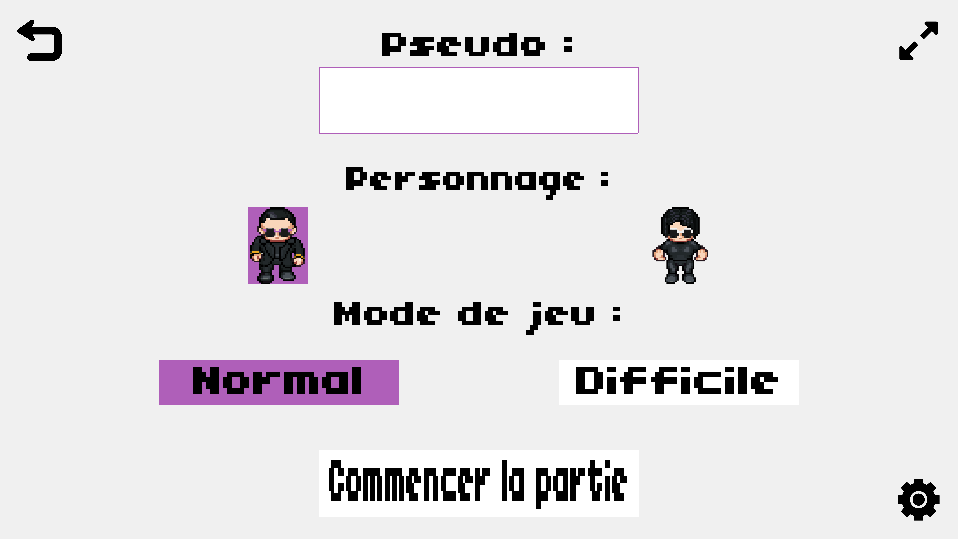
\includegraphics[width=10cm]{images/nouvelle_partie.png}\\

                \newpage

                \item \tabto{1cm} \underline{Les options~:}\\\\
                \tabto{1cm} En cliquant sur le bouton «~Options~», le joueur accède à une nouvelle page où il pourra changer différents paramètres contenus dans deux onglets différents. On peut y retrouver l’onglet «~Son~» où la modification du son de la musique et celle des effets sonores est possible. De plus, on peut accéder à l’onglet «~Touches~» où le joueur peut modifier les touches pour aller à droite, pour aller à gauche, pour sauter ou monter, pour descendre et celle pour intéragir.\\

                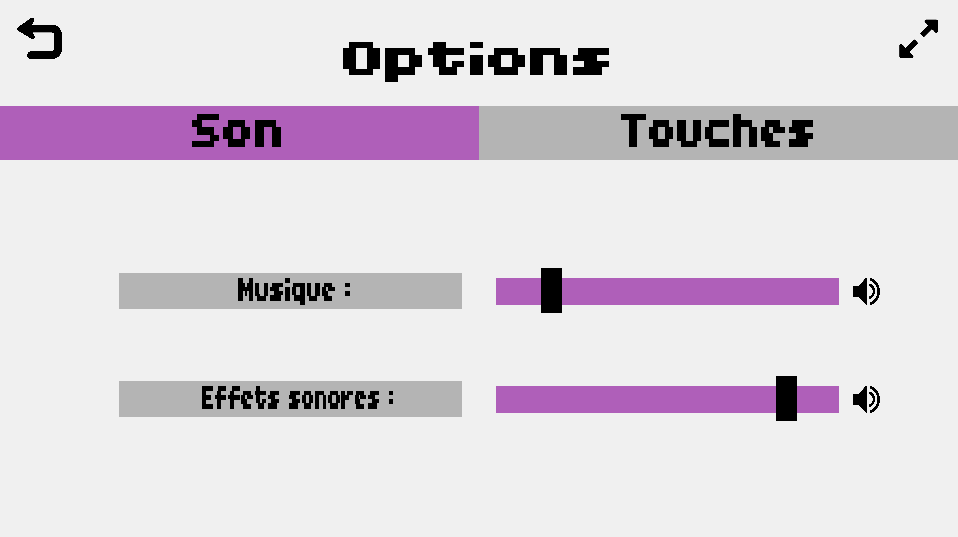
\includegraphics[width=5cm]{images/options_son.png}
                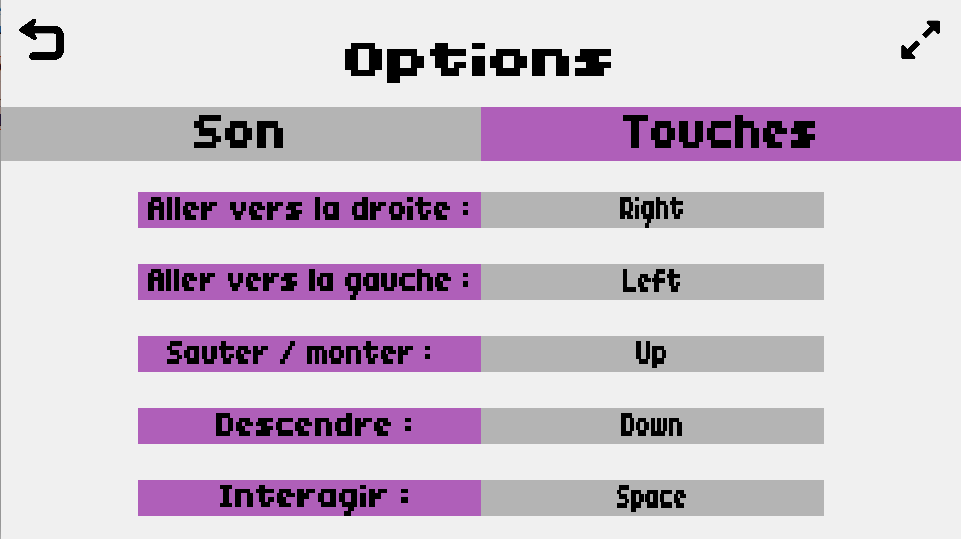
\includegraphics[width=5cm]{images/options_touches.png}\\
                
                \item \tabto{1cm} \underline{La carte~:}\\\\
                \tabto{1cm} Puis en cliquant sur le bouton «~Continuer~», le joueur accède à l’onglet central du jeu où il peut se déplacer sur la carte du monde pour choisir le niveau auquel il veut jouer. Il est possible d'observer l’image de fond qui représente la carte et qui possède quatre niveaux. Au début d’une partie, le joueur est au premier niveau mais n’a pas accès aux niveaux suivants. Ils se débloquent au fur et à mesure que l’utilisateur termine les niveaux.\\

                
\includegraphics[width=10cm]{images/carte.png}\\
                
            \end{itemize}

            \newpage

            \tabto{1cm} La navigation dans notre projet est toujours la même et permet de d'accéder directement à la plupart des onglets rapidement et sans difficulté.\\

            \begin{figure}[h]
                \centering
                \includegraphics[width=13cm]{images/schéma_navigation.png}\\
            \end{figure}

            Pour plus d'informations, voir le schéma détaillé dans l'annexe : \ref{subsec:schéma_navigation_detaille}\\

            \tabto{1cm} De plus, les quatre niveaux auxquels le joueur peut jouer demandent des mécaniques souvent différentes pour pas que l’utilisateur ne perde l’envie de jouer au bout d’un certain temps. Dans tous les niveaux et en particulier dans le premier et le dernier, le joueur doit utiliser les touches pour aller vers la droite, vers la gauche et pour sauter afin de pouvoir déplacer le personnage. Cependant, dans les mini-jeux des deuxième et troisième niveaux, ces touches ne correspondent pas exactement au déplacement du personnage comme on pouvait le voir jusqu’à présent. Dans le premier mini-jeu du second niveau, l’objectif et de relier des tuyaux entre eux pour faire un chemin. Le joueur utilisera les touches principales pour se déplacer de tuyau en tuyau et la touche d’interaction pour tourner ces derniers. Nous pouvons retrouver cette mécanique dans le second mini-jeu du troisième niveau, qui va juste demander en plus au joueur de rester appuyé sur la touche d’interaction, pour pouvoir bouger un bloc du départ à l’arrivée et tout ceci dans un labyrinthe. Pour finir, dans le premier mini-jeu du troisième niveau, le joueur reconstitura un composant qui est divisé en plusieurs parties. Il devra seulement utiliser la souris pour y parvenir.\\
 
    \newpage

    \section{Outils et méthodes utilisés pour le codage}
        \tabto{1cm} Dans cette partie, nous allons traiter l'onglet centrale de notre projet, qui regroupe les outils utilisés et l'écriture du code.

        \subsection{Les différents outils exploités}
            \tabto{1cm} Avant de commencer le codage, nous avons pris connaissance de différents outils que nous allons vous présenter tout en détaillant leur fonctionnement~:\\
            
            \begin{itemize}
                \item Visual Studio Code 1.81.1
                \item GitHub 2.25.1
                \item GCC  9.4
                \item Valgrind 3.15
                \item Débogueur GDB 9.2
                \item LaTeX 3.14
                \item Google Drive
            \end{itemize}

             \subsubsection{Visual Studio Code}
                \tabto{1cm} Visual Studio Code est l’outil de développement principal que nous avons utilisé, notamment pour ses diverses extensions et son intégrité qui nous a permis de mieux exploiter certains outils supplémentaires~:\\

                \newpage
                
                \begin{itemize}
                    \item Doxygen~: mettre en forme les commentaires sous forme de Doxygen\\

                    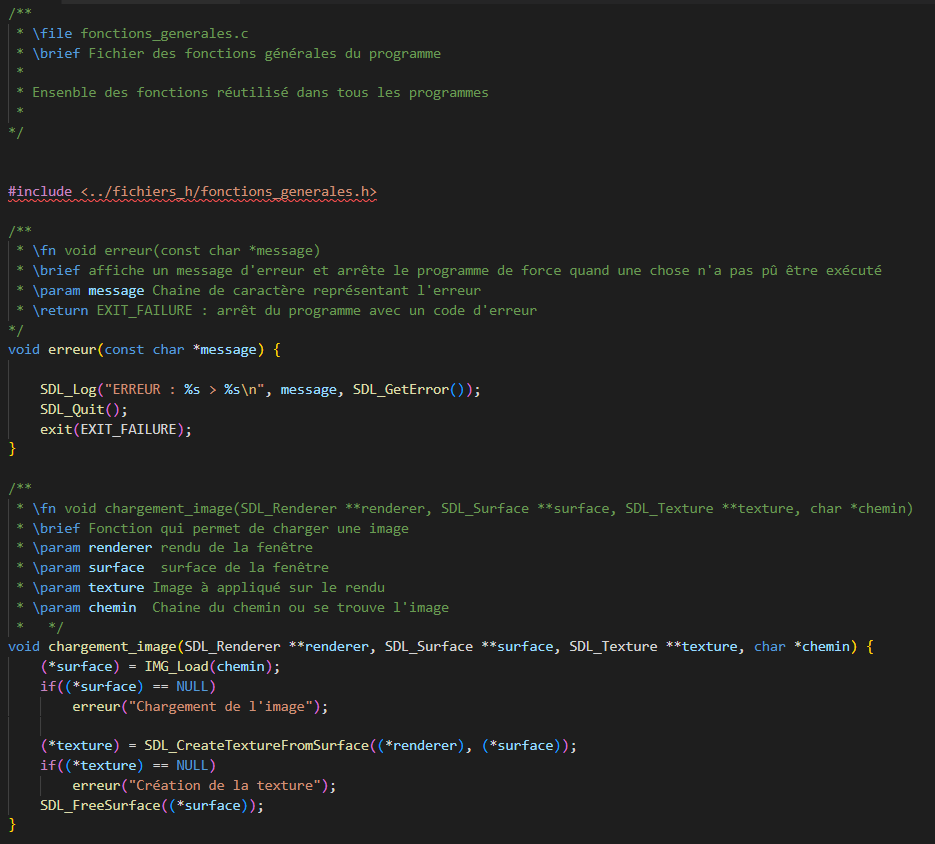
\includegraphics[width=10cm]{images/doxygen.png}\\

                    Pour plus d'informations, voir le Doxygen dans l'annexe : \ref{subsec:doxygen}.\\
                    
                    \item GitHub Pull Request~: permet d’appliquer les commandes GitHub à partir de Visual Studio Code de manière rapide
                \end{itemize}
                
            \subsubsection{GitHub}
                \tabto{1cm} GitHub est le premier outil que nous avons appris à manipuler et à utiliser pour mettre notre code en commun. Cet outil fournit beaucoup de possibilités d’organisation, tel que la création de différentes branches et la faculté de fusion. Des complications dûes à notre manque de connaissance sur cet outil et différents problèmes rencontrés nous ont fait perdre du temps. Nous avons donc décidé de limiter l’usage de GitHub pour tirer et pousser nos travaux dans la branche principal, laissant une sauvegarde de côté en cas de soucis sur le code principal.

            \subsubsection{GCC}
                \tabto{1cm} GCC a été choisi comme compilateur dû à sa capacité à créer des versions «~.o~» de nos programmes, permettant une compilation plus rapide des~modules.
            
            \subsubsection{Valgrind}
                \tabto{1cm} L’usage de Valgrind nous a permis la détection des différentes fuites de mémoire et du bon usage des pointeurs (hors usage de la bibliothèque SDL qui en produit naturellement). Cet outil nous a fourni une bonne détection des erreurs d’usage des pointeurs, notamment les erreurs de segmentation et des fuites de mémoire liées à l’oubli de la commande «~free~» après une allocation dynamique.
                
            \subsubsection{GDB}
                \tabto{1cm} GDB est un outil de débogage que nous avons utilisé pour identifier des erreurs lors de nos tests sur plusieurs entités, surtout liées à l’utilisation de la bibliothèque SDL. Vous pouvez voir ci-dessous une utilisation de cet outil permettant de comprendre où se situait l’erreur de segmentation lors de l’appel d’une fonction.\\

                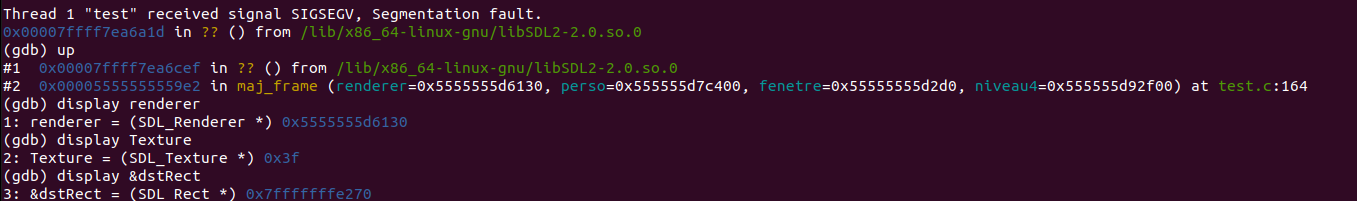
\includegraphics[width=13cm]{images/debogage.png}\\
                
            \subsubsection{Google Drive}
                \tabto{1cm} Nous avons utilisé cet outil pour la mise en commun de nos idées, pour l’utilisation du diagramme de Gantt et pour le cahier des charges.

        \subsection{La méthode \textit{tilemap}}
            \tabto{1cm} À travers les nombreuses mécaniques employées dans notre code, l’utilisation du \textit{tilemap} est l’une des parties les plus cruciales. La méthode \textit{tilemap}, appelée aussi «~la carte par tuile~» est une méthode largement utilisée dans le domaine du jeu vidéo et dans la simulation graphique grâce à ses avantages sur la mémoire (petit coût par rapport au chargement d’image), mais aussi sur son utilisation (facilement utilisable et exploitable). Chaque \textit{tilemap} utilise une matrice qui est remplie de valeurs numériques et dont la taille varie (en fonction de son utilité). Ces valeurs possèdent chacune une texture unique qui leur est assignée. Lors de l’affichage de la partie graphique, les données de chaque tuile ne sont pas sauvegardées mais actualisées en fonction de leur position dans la matrice. La \textit{tilemap} est le centre d’interaction entre les informations reçues par le joueur dans les niveaux et le bon déroulement du programme.\\
	
        	\tabto{1cm} Malgré les avantages de la méthode \textit{tilemap}, nous pouvons constater que cette technique dispose de quelques limites. La \textit{tilemap}, ne pouvant pas laisser place à un système de génération automatique, est créée manuellement nécessitant une rigueur dans la construction de la matrice. Cette dernière ne procure qu’un seul moyen pour afficher les éléments au travers de la SDL et en aucun cas ne peut s’occuper d’un autre système, tel que celui de la collision ou de la reconnaissance de texture.

         \subsection{Les différentes structures et fonctions générales}
            \tabto{1cm} Pour lier nos travaux et avoir une bonne organisation du code, nous avons utilisé diverses structures et énumérations. Ainsi, nous utilisons les mêmes noms de ces dernières pour avoir une meilleure fusion des modules du programme. Voici un échantillon des différentes structures et énumérations que nous avons utilisées~:\\

            \begin{itemize}
                \item barreDeSon~: gère l’aspect du son
                \item page\textunderscore t~: permet de savoir sur quelle page on se trouve
                \item position\textunderscore t~: donne la position du personnage sur la carte
                \item direction\textunderscore t~: donne la direction du personnage sur la carte\\
            \end{itemize}

            Nous avons aussi implémenté des fonctions communes tel que~:\\
            
            \begin{itemize}
                \item erreur~: fonction qui arrête le programme en cas d’erreur et retourne un message correspondant
                \item chargement\textunderscore image~: charge une image dans une texture
            \end{itemize}

        \newpage
        
         \subsection{La gestion des niveaux et des mini-jeux}   
            \tabto{1cm} Les niveaux sont stockés dans des structures, qui sont elles-mêmes représentées par des pointeurs et des variables, servant à la représentation des différents éléments du niveau.\\

            \tabto{1cm} Parmi les obstacles notoires que nous avons rencontré dans le développement de nos mini-jeux, l’implémentation de ces derniers dans notre programme principal et l'empêchement des conflits de comportement ont été les plus difficiles et les plus longs à résoudre. Nous pouvons prendre l'exemple que lorsque le mini-jeu était isolé à son propre programme, celui-ci se comportait correctement tandis que lors de son implémentation au programme principal, il présentait des comportements anormaux (mauvais déplacement, erreurs de segmentation, bugs, etc). Malgré les outils mis à notre disposition (Valgrind, GDB), certains problèmes étaient difficilement détectables par ces derniers. Cela était majoritairement dû à des erreurs de signe ou d’assignation de variables subtiles. Nous pouvons prendre l'exemple du mini-jeu de la tuyauterie, lors de la vérification du trajet où il y avait des erreurs sur les modifications de coordonnées. Par conséquent, la complexité de certains niveaux a été remise en question soit à cause d’un nombre de calcul trop grand, tel que la tuyauterie qui faisait trop d’appels récursifs pour tester toutes les combinaisons possibles, soit à cause de certains paternes qui faisaient des boucles infinies pendant la vérification du chemin.
            
         \subsection{Les tests unitaires}
            \tabto{1cm} L’objectif des tests unitaires est de vérifier l’intégralité et le bon déroulement d’une fonction ou d’une structure de donnée sans être biaisée par d’autres (c’est à dire prendre en compte les erreurs potentielles induites par des fonctions extérieures à une autre ou à une structure de donnée initiale).

            \subsubsection{Test unitaire du pseudo}
                \tabto{1cm} Le test unitaire le plus important qui nous a permis de trouver le plus grand nombre d'erreurs dans notre code a été celui de la saisie du pseudo dans l'onglet «~Nouvelle Partie~». Il possède un grand nombre de conditions qui permet au pseudo d'être valide.\\
                Pour plus d'informations, voir le test unitaire du pseudo dans l'annexe : \ref{subsec:test_unitaire_pseudo}.
                
            \subsubsection{Création des mini-jeux}
                \tabto{1cm} Afin de tester l’agencement de nos mini-jeux, nous avons créé un algorithme permettant d’avoir un suivi sur leurs comportements. La création de ces derniers à partir d’un fichier externe ont permis de tester différents paternes de jeu afin de prévoir des comportements qui pourraient poser plusieurs problèmes et la destruction de ces derniers (mise à «~NULL~»). En parallèle, nous avons fait appel à des personnes extérieures au projet, avec aucune connaissance du jeu et des règles, afin de tester les limites de nos mini-jeux. Ceci nous a permis de détecter plusieurs erreurs graphiques et pratiques. Par la même occasion, cela nous a permis de s’assurer qu’aucune fuite de mémoire était présente.
            
    \newpage

    \section{Résultat et conclusion}
        \tabto{1cm} Dans cette conclusion, nous présentons le résultat obtenu ainsi qu'un bilan de notre expérience dans le développement de notre jeu.\\

        \subsection{Résultat du projet}
            \tabto{1cm} Notre jeu, fruit de nombreuses heures de travail et de dévouement, fonctionne avec succès. Nous avons réussi à créer un environnement de jeu immersif et engageant, offrant aux joueurs une expérience divertissante et captivante. Cependant, malgré notre satisfaction initiale, nous avons identifié plusieurs aspects à améliorer pour enrichir davantage l'expérience des utilisateurs. Parmi ces améliorations figurent l'ajout de nouveaux niveaux pour étendre la durée de jeu, la possibilité de jouer à la manette pour offrir une alternative de contrôle plus intuitive, ainsi que l'introduction d'un système de vie pour augmenter le défi et la tension du jeu.\\
            
            En outre, notre planification initiale a été perturbée par nos obligations personnelles et scolaires, notamment nos cours et nos partiels. Le manque de temps disponible a entravé notre capacité à respecter pleinement notre emploi du temps, retardant ainsi certaines tâches et fonctionnalités prévues. De plus, la découverte et la prise en main de la bibliothèque SDL ont pris plus de temps que prévu, retardant ainsi le développement global du jeu. Enfin, la répartition des rôles s'est faite au fur et à mesure de nos réunions, ce qui a parfois entraîné des retards et des conflits de vision.\\

        \subsection{Bilan du projet}
            \tabto{1cm} Malgré les problèmes rencontrés, cette expérience de développement de jeu a été incroyablement enrichissante. Nous avons acquis une compréhension plus approfondie du processus de développement de jeux vidéo, ainsi qu'une appréciation du travail d'équipe et de la résolution de problèmes. Nous aimerions continuer cette aventure et améliorer notre jeu avec une base solide dans le langage de programmation, ainsi qu'une planification plus réaliste et une gestion plus efficace du temps. Nous sommes reconnaissants pour cette opportunité et impatients de voir où nous mènera cette expérience dans le futur.

    \section{Annexe}

        \subsection{Schéma détaillé de la navigation}
            \label{subsec:schéma_navigation_detaille}
            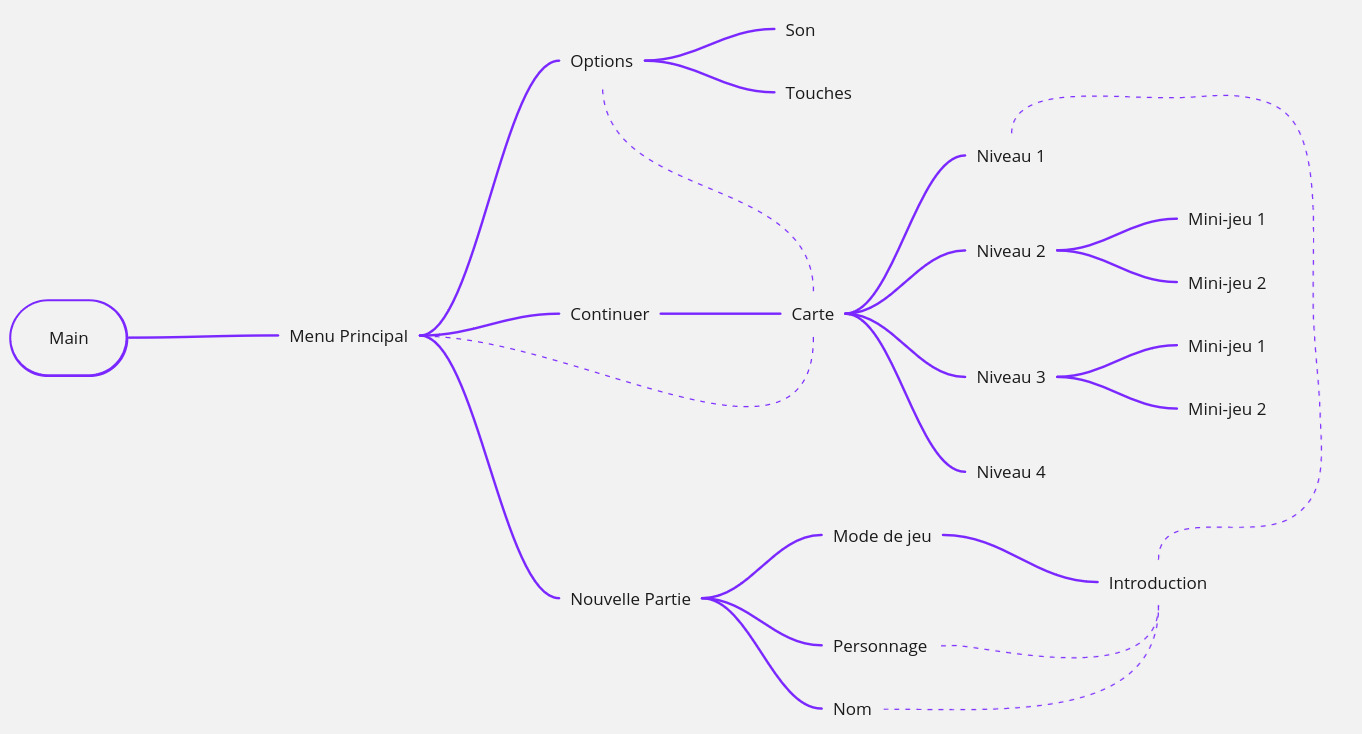
\includegraphics[width=13cm]{images/schéma_navigation_détaillé.png}

        \newpage

        \subsection{Doxygen}
            \label{subsec:doxygen}
            
            \begin{center}
                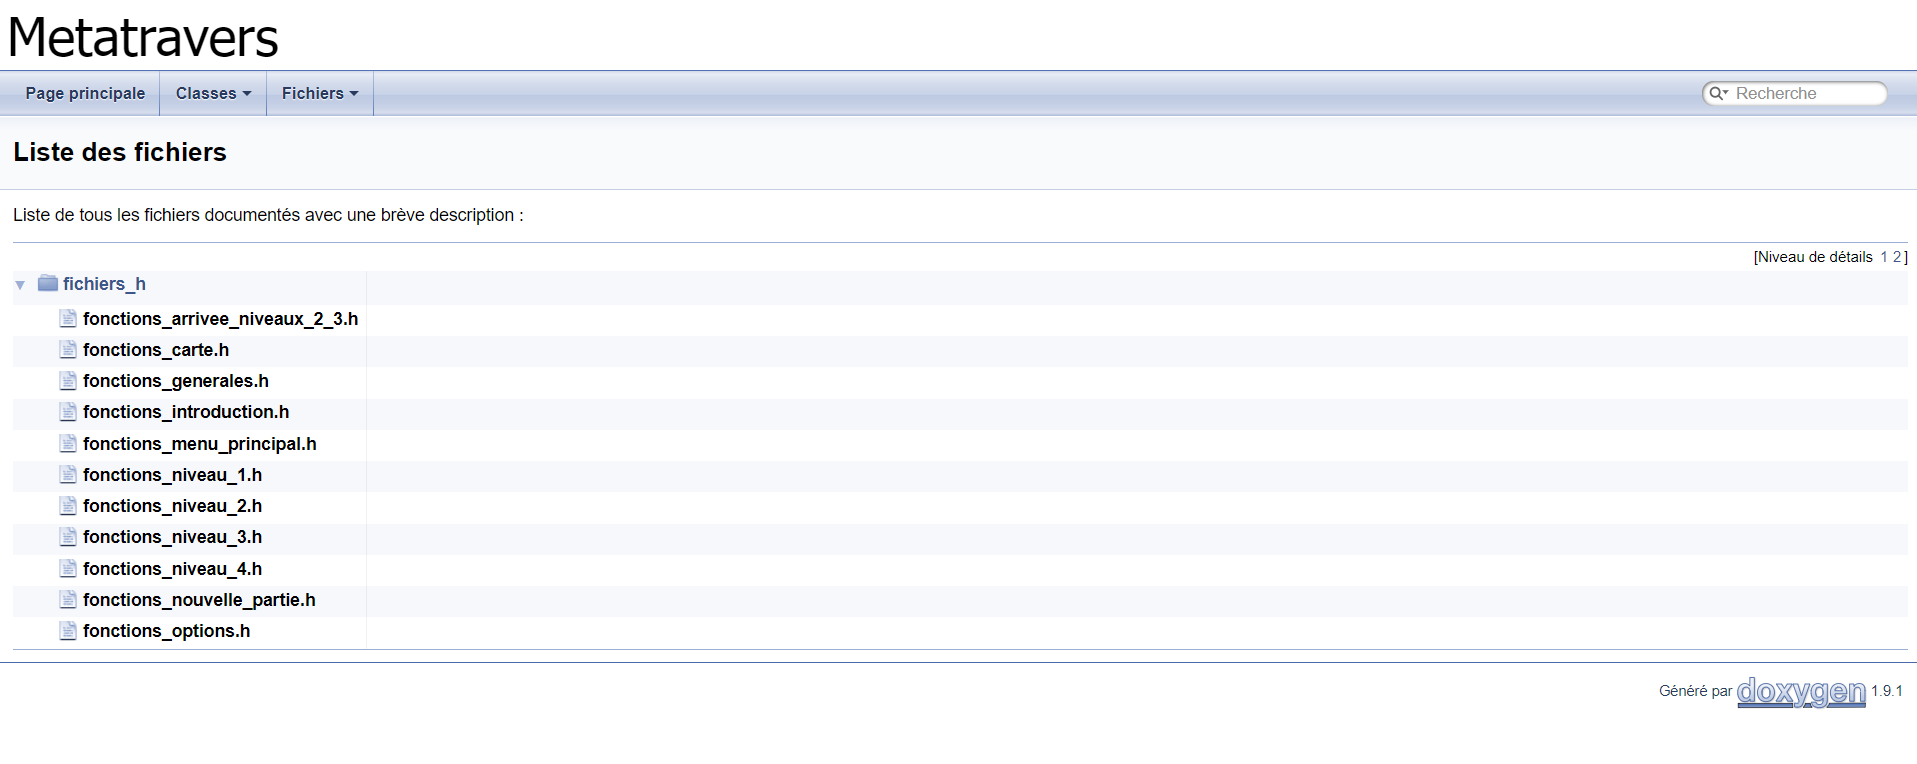
\includegraphics[width=13cm]{images/doxygen_html.png}\\
                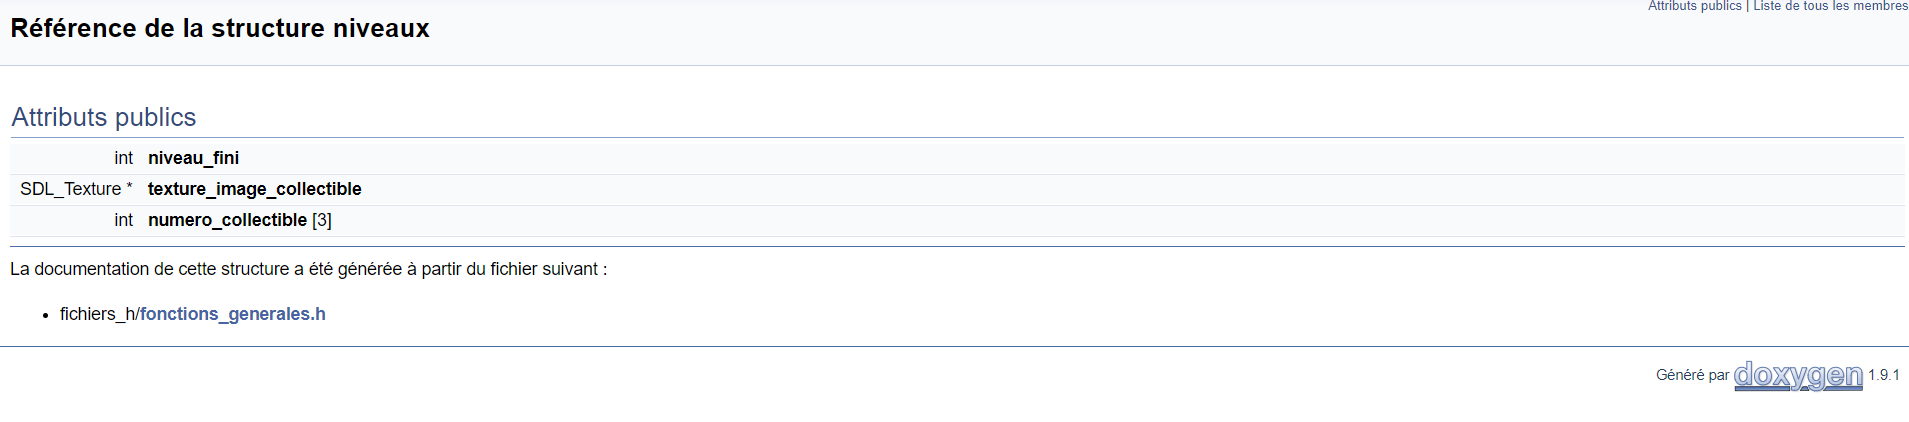
\includegraphics[width=13cm]{images/doxygen_niveau.png}\\
                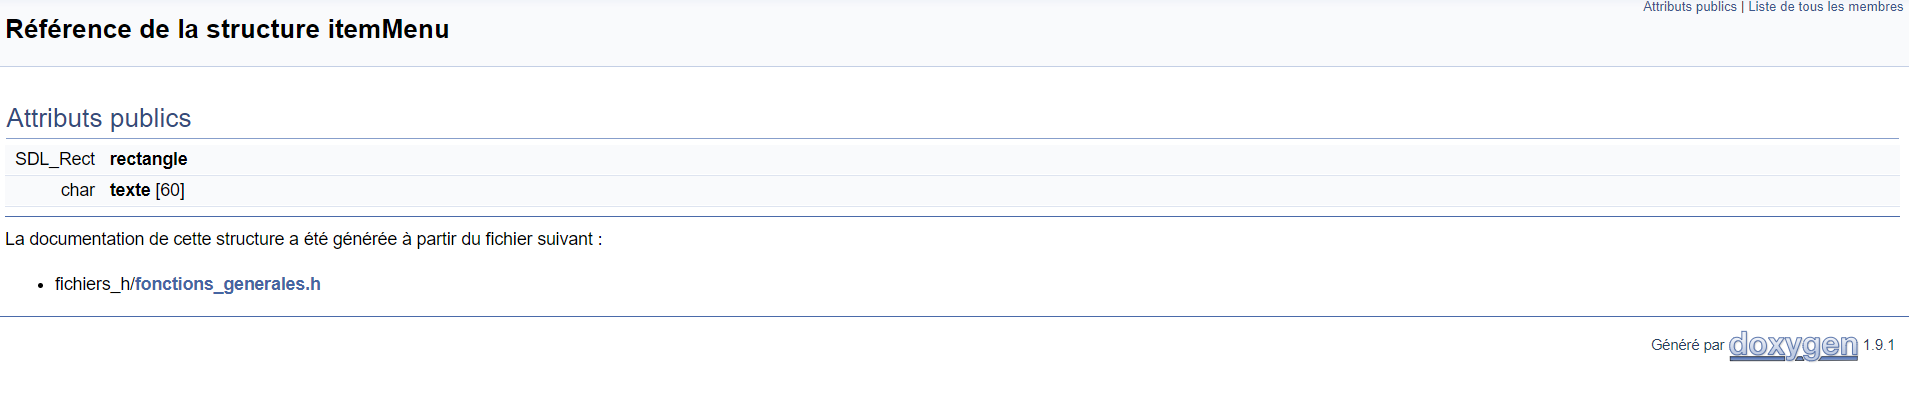
\includegraphics[width=13cm]{images/doxygen_itemMenu.png}\\
                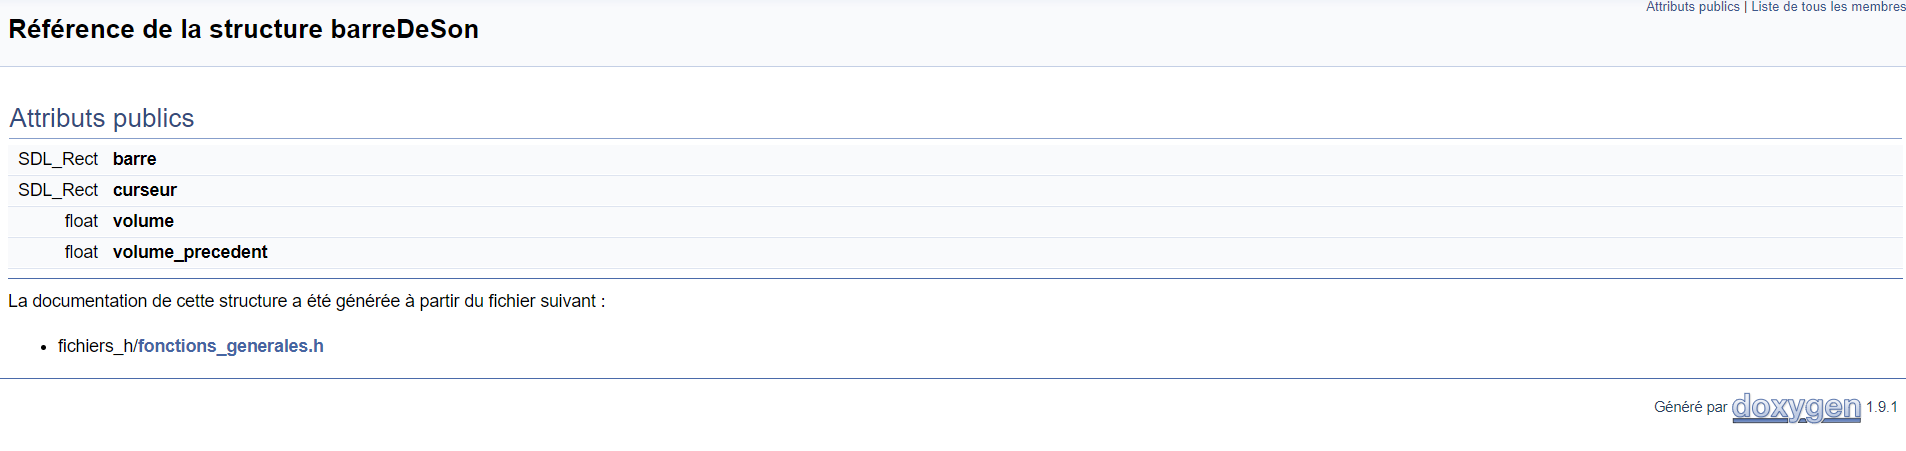
\includegraphics[width=13cm]{images/doxygen_barreDeSon.png}
            \end{center}
            
        \subsection{Test unitaire du pseudo}
            \label{subsec:test_unitaire_pseudo}
            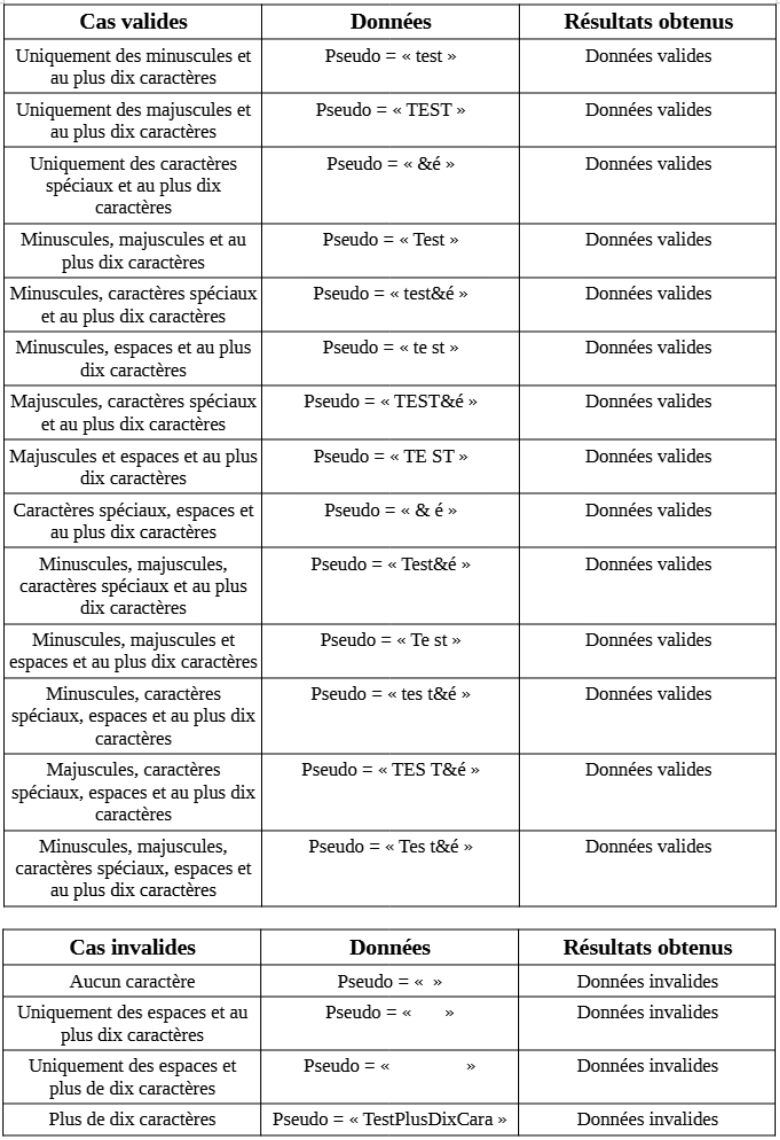
\includegraphics[width=13cm]{images/test_unitaire_pseudo.png}

\end{document}
